\chapter{Termodinámica}

El calor es un proceso de transmisión, es decir que fluye de un punto de mayor temperatura a una de menor 
temperatura. El concepto de gradiente es fundamental:

\begin{definition}[Gradiente]
    Es una magnitud física que relaciona la variación de temperatura por unidad de distancia. En el sistema internacional su unidad de medida es el Kelvin/metro. 
\end{definition}

\section{Variables termodinámicas}

Una variable es una propiedad de la materia que es susceptible a variar, en función de algún motivo determinado o indeterminado. 

La variabilidad se debe a la poca estabilidad, lo que permite cambios en el tiempo como sería el clima o incluso en el humor. 


Existen ciertos tipos de variables:  

\begin{enumerate}
    \item Dependiente: Depende de otra variable 
    \item Independiente: No depende de otra variable    
    \item Discreta: El dato toma estados fijos dentro del tiempo  
    \item Continua: Puede variar en el tiempo.
\end{enumerate}

El valor de una variable extensiva depende del tamaño del sistema (Masa, volumen, energía interna, etc\dots). mientras que el valor de una variable intensiva no depende del tamaño ni de la cantidad de materia del sistema (color, temperatura, dureza\dots).

La temperatura depende de la humedad relativa, la presión depende de una bomba o de la gravedad. Pero los gases 
tienen cierta propiedades también: 

El aire es un gas, está compuesto de 78\%, 21\% oxígeno, 0.03\% de $CO_2$ y el resto son gases raros:

\begin{itemize}
    \item Densidad $(r)$
    \item Volumen específico $(v)$
    \item Presión $(p)$
    \item Temperatura $(T)$
    \item Viscosidad $(\mu)$
    \item Gas constante $(R)$
    \item Calor específico $(c_v)$
    \item Ratio $(\gamma)$
\end{itemize}

\begin{definition}[Volumen específico]
    Es el volumen ocupado por unidad de masa de un material. Es el inverso de la densidad, por lo cual no dependen de la cantidad de materia.
\end{definition}

Dos pedazos de aluminio de diferente tamaño ocupan diferente volumen y no pesan igual, pero su volumen específico es igual.

\begin{align}
    &v=\frac{V}{m}\left(\frac{m^3}{Kg}\right)\\ 
    &\rho=\frac{1}{v}\left(\frac{Kg}{m^3}\right)
\end{align}

\section{Primera Ley de la Termodinámica}

Todos los seres vivos dependen de la energía para sobrevivir, y las civilizaciones modernas
continuar prosperando solo si las fuentes de energía existentes pueden desarrollarse para satisfacer
las crecientes demandas. La energía existe en muchas formas, desde la energía encerrada en
los átomos de la materia misma a la intensa energía radiante emitida por el sol.
Existen muchas fuentes de energía; muchos son conocidos, algunos quizás desconocidos; pero
cuando existe una fuente de energía, primero se deben encontrar los medios para transformar la energía
en una forma conveniente a nuestro propósito.

La energía química de la combustión de combustibles fósiles (petróleo, carbón, gas) y desechos.
(agrícola, industrial, doméstico), se utiliza para producir calor que a su vez se utiliza
para proporcionar energía mecánica en turbinas o motores alternativos; uranio
los átomos se bombardean en dos y la energía nuclear liberada se utiliza como calor;
la energía potencial de grandes masas de agua se convierte en energía eléctrica
al pasar por turbinas de agua en su camino desde las montañas hasta el mar;
la energía cinética del viento es aprovechada por molinos de viento para producir electricidad;
la energía de las olas del mar se convierte en energía eléctrica en flotación
turbinas; las mareas producidas por la rotación de la luna producen electricidad
energía al fluir a través de turbinas en grandes estuarios fluviales; rocas calientes y
Los líquidos atrapados en las profundidades de la tierra están hechos para liberar su energía a
convertirse en electricidad; la inmensa energía radiante del sol se aprovecha para
El agua caliente o mediante un dispositivo adecuado se convierte directamente en electricidad. Figura \ref{te8}
muestra las diversas fuentes de energía y las posibles rutas de conversión con el
las transferencias más importantes se muestran como líneas en negrita; 


\begin{figure}[h!]
    \centering
    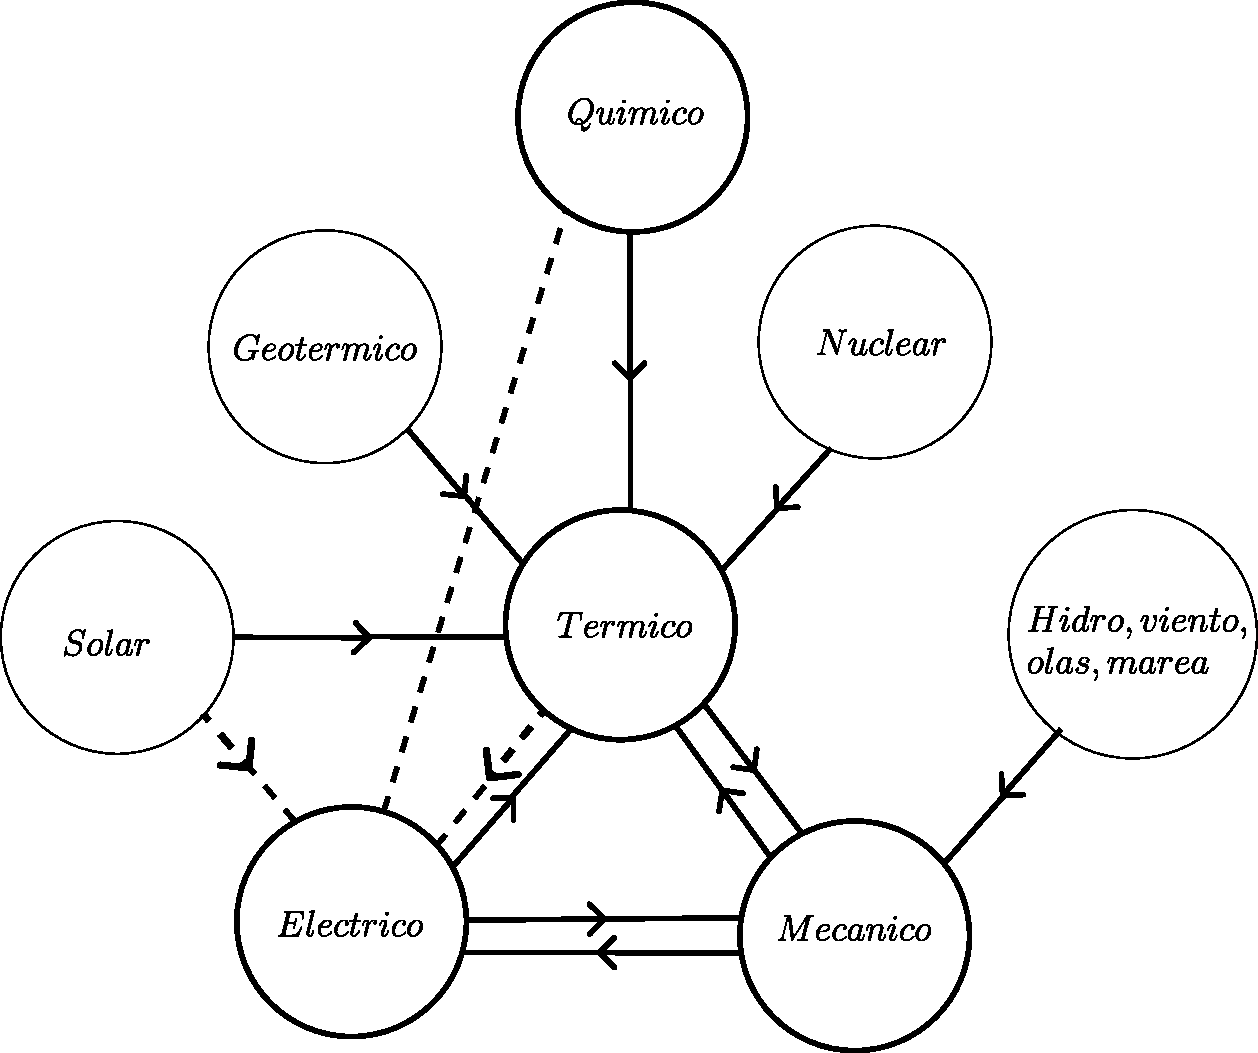
\includegraphics[scale=0.5]{te8.pdf}
    \caption{Conversión de energía}
    \label{te8}
\end{figure}



\begin{definition}[Termodinámica aplicada]
    es la ciencia de la relación entre calor, trabajo,
y las propiedades de los sistemas.
\end{definition}

Se ocupa de los medios necesarios para convertir la energía térmica de las fuentes disponibles, 
como los combustibles fósiles, en mecánica
trabajo, Un motor térmico es el nombre que se le da a un sistema que al operar en un
La forma cíclica produce trabajo neto a partir de un suministro de calor. Las leyes de
La termodinámica son hipótesis naturales basadas en observaciones del mundo en
que vivimos. Se observa que el calor y el trabajo son dos factores mutuamente convertibles
formas de energía. y esta es la base de la Primera Ley de la Termodinámica. Eso
También se observa que el calor nunca fluye sin ayuda de un objeto a baja temperatura.
temperatura a una temperatura alta, de la misma manera que un río nunca fluye cuesta arriba sin ayuda. 
Esta observación es la base de la \textbf{Segunda Ley de Termodinámica}, que se puede utilizar para demostrar que una máquina 
térmica no puede convertir todo el calor que se le suministra en trabajo mecánico, pero siempre debe rechazar algunos
calentar a una temperatura más baja. Estas ideas serán discutidas y desarrolladas en
a su debido tiempo, pero primero deben hacerse algunas definiciones fundamentales.

\subsection{Calor, trabajo y sistema}

Para tratar el tema de la termodinámica aplicada de manera rigurosa es
necesario para definir los conceptos utilizados.

El calor es una forma de energía que se transfiere de un cuerpo a otro.
a una temperatura más baja, en virtud de la diferencia de temperatura entre el
cuerpos.

Por ejemplo, cuando un cuerpo $A$ en una cierta temperatura, digamos 20 $C^{\circ}$, se lleva
en contacto con un cuerpo $B$ a una temperatura más alta, digamos 21 $C^{\circ}$, entonces habrá
ser una transferencia de calor de $B$ a $A$ hasta que las temperaturas de $A$ y $B$ sean iguales
(Figura \ref{te9}). Cuando la temperatura de $A$ es la misma que la temperatura de $B$ no
la transferencia de calor tiene lugar entre los cuerpos, y se dice que están en temperatura
equilibrio. El calor es aparente sólo durante el proceso y por lo tanto es transitorio
energía. Dado que la energía térmica fluye de $B$ a $A$, hay una reducción en la intrínseca
energía poseída por $B$ y un aumento en la energía intrínseca poseída por $A$.
Esta energía intrínseca de un cuerpo, que es al menos una función de la temperatura,
no debe confundirse con el calor. El calor nunca puede estar contenido en un cuerpo o
poseído por un cuerpo.

\begin{figure}[h!]
    \centering
    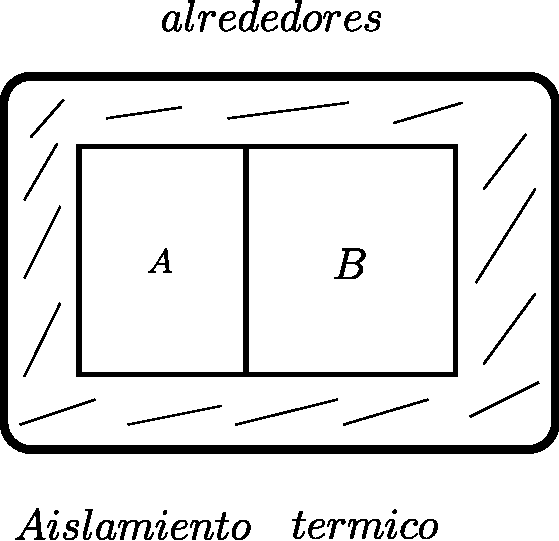
\includegraphics[scale=0.5]{te9.pdf}
    \caption{Dos aislados cuerpos en contacto}
    \label{te9}
  \end{figure}

Un sistema puede definirse como una colección de materia dentro de los límites prescritos y
límites identificables. Los límites no son necesariamente inflexibles;
por ejemplo, el fluido en el cilindro de un motor alternativo durante la

Para tratar el tema de la termodinámica aplicada de manera rigurosa es
necesario para definir los conceptos utilizados.

\begin{definition}[Calor]
    Es una forma de energía que se transfiere de un cuerpo a otro.
a una temperatura más baja, en virtud de la diferencia de temperatura entre el
cuerpos.
\end{definition}

la carrera de expansión se puede definir como un sistema cuyos límites son las paredes del cilindro
y la corona del pistón. A medida que se mueve el pistón, también se mueven los límites.
Este tipo de sistema se conoce como sistema cerrado.

Un sistema abierto es aquel en el que hay una transferencia de masa a través del
límites; por ejemplo, el fluido en una turbina, en cualquier instante puede definirse
como un sistema abierto.

La presión de un sistema es la fuerza ejercida por el sistema sobre el área de la unidad
de sus límites. Las unidades de presión son, por ejemplo, pascal, $Pa$ (donde
$1 Pa = 1 \frac{N}{m^2}$), o \texttt{bar}; el símbolo $p$ se utilizará para la presión. Presión como
definido aquí se llama presión absoluta. Un manómetro para medir la presión,
registra la presión por encima de la atmosférica. Esto
se llama presión manométrica, la presión absoluta es igual a la presión manométrica más
presión atmosférica.

\subsubsection{Presión}

La unidad de presión (fuerza por unidad de área) es $\frac{N}{m^2}$ y esta unidad es a veces
llamado pascal, Pa. Para la mayoría de los casos que ocurren en termodinámica, la presión
expresado en pascales sería un número muy pequeño; una nueva unidad se define como
sigue:

\begin{equation}
    1 bar = 105\frac{N}{m^2} = 10^{\circ} Pa
\end{equation}

La ventaja de usar una unidad como la barra es que es aproximadamente igual
a la presión atmosférica. De hecho, la presión atmosférica estándar es exactamente
1,01325 \texttt{bar}.

A menudo es conveniente expresar una presión como cabeza de un líquido. Tenemos:

Presión atmosférica estándar = 1.01325 \texttt{bar} = 0.76m Hg

\subsubsection{Temperatura}

La variación de una propiedad fácilmente medible de una sustancia con la temperatura.
se puede utilizar para proporcionar un instrumento de medición de temperatura. Por ejemplo, el
la longitud de una columna de mercurio variará con la temperatura debido a la expansión
y contracción del mercurio. El instrumento se puede calibrar marcando
la longitud de la columna cuando se pone en equilibrio térmico con el
vapor de agua hirviendo a presión atmosférica y nuevamente cuando está en temperatura
equilibrio con hielo a presión atmosférica. En grados Celsius (o centígrados)
escala Se hacen 100 divisiones entre los dos puntos fijos y se toma el cero
en el punto de hielo.

El cambio de volumen a presión constante, o el cambio de presión a
volumen constante, de una masa fija de gas que no se licua fácilmente (por ejemplo, oxígeno,
Hidrógeno, helio, etc.) Se puede utilizar como medida de temperatura. Tal
El instrumento se llama termómetro de gas. [t se encuentra para todos los gases utilizados en
termómetros que si el gráfico de temperatura contra volumen en el
El termómetro de gas a presión constante se extrapola más allá del punto de hielo al
punto en el que el volumen del gas se volvería cero, entonces la temperatura
en este punto es de —273 $C^{\circ}$ aproximadamente. Del mismo modo, si la gráfica de
La temperatura contra la presión en el termómetro de gas de volumen constante es
extrapolado a presión cero, entonces se encuentra el mismo cero de temperatura. Un
Por lo tanto, se ha fijado el cero absoluto de temperatura y se ha establecido una escala absoluta de
se puede definir la temperatura. La temperatura en la escala Celsius absoluta se puede
ser obtenido sumando 273 a todas las temperaturas en la escala de celsius.

\subsection{El estado del fluido de trabajo}

En todos los problemas de termodinámica aplicada nos ocupamos de las transferencias de energía
hacia o desde un sistema. En la práctica, el asunto contenido en el
Los límites del sistema pueden ser líquido, vapor o gas, y se conoce como
trabajando fluidamente. En cualquier instante, el estado del fluido de trabajo puede definirse por
ciertas características llamadas sus propiedades. Muchas propiedades no tienen importancia
en termodinámica (por ejemplo, resistencia eléctrica), y no se considerará. La
Las propiedades termodinámicas presentadas en este libro son presión, temperatura,
volumen específico, energía interna específica, entalpía específica y entropía específica.
Se ha encontrado que, para cualquier fluido de trabajo puro, solo dos
Las propiedades son necesarias para definir completamente el estado del fluido. Dado que cualquier
dos propiedades independientes son suficientes para definir el estado de un sistema, es posible
representar el estado de un sistema mediante un punto situado en un diagrama de propiedades.
Por ejemplo, un cilindro que contiene un cierto fluido a la presión $p$, y específico
volumen $v_1$, está en el estado 1, definido por el punto 1 en un diagrama de $p$ contra $pv$. 
Dado que el estado está definido, entonces la temperatura del fluido, $T$, es
fijo y el punto de estado se puede ubicar en un diagrama de $p$ contra $T$ y $T$
contra $v$. En cualquier otro instante, el pistón puede
moverse en el cilindro de manera que la presión y el volumen específico cambien.
A continuación, se puede marcar el estado 2 en los diagramas. Los diagramas de propiedades se utilizan continuamente en termodinámica aplicada para graficar los cambios de estado. El más importantes son los diagramas de presión-volumen y temperatura-entropía, pero
Los diagramas de entalpía — entropía y presión — entalpía también se utilizan con frecuencia.

\subsection{Reversibilidad}

Se demostró que el estado de un fluido se puede representar mediante un
punto ubicado en un diagrama usando dos propiedades como coordenadas. Cuando un sistema
cambia de estado de tal manera que en cualquier instante durante el proceso el estado
punto se puede ubicar en el diagrama, entonces se dice que el proceso es reversible.
El fluido que experimenta el proceso pasa a través de una serie continua de
estados de equilibrio. Por tanto, un proceso reversible entre dos estados puede ser
trazada como una línea en cualquier diagrama de propiedades. 

En la práctica, el fluido que experimenta un proceso no puede mantenerse en equilibrio en su fase intermedia.
estados y una ruta continua no se pueden trazar en un diagrama de propiedades. Semejante
Los procesos verde azulado se denominan procesos irreversibles. Un proceso irreversible suele ser
representado por una línea de puntos que une los estados finales para indicar que
los estados intermedios son indeterminados.

\begin{definition}[Reversibilidad]
    Cuando un fluido se somete a un proceso reversible, tanto el fluido como su entorno
siempre se puede restaurar a su estado original.
\end{definition}


Los criterios de reversibilidad son los siguientes:

\begin{enumerate}
    \item El proceso debe ser sin fricción. El fluido en sí no debe tener fricción interna.
    y no debe haber fricción mecánica (por ejemplo, entre cilindro y pistón).
    \item La diferencia de presión entre el fluido y su entorno durante el
    El proceso debe ser infinitamente pequeño. Esto significa que el proceso debe tener lugar
    infinitamente lento, ya que la fuerza para acelerar los límites del sistema
    es infinitamente pequeño.
    \item  La diferencia de temperatura entre el fluido y su entorno durante
    el proceso debe ser infinitamente pequeño. Esto significa que el calor suministrado o
    rechazado hacia o desde el fluido debe transferirse infinitamente lentamente.
\end{enumerate}


%%%%%%%%%%%%%%%%%%%%%%%%%%%%%%%%%%%%%%%%%%%%%%%%%%%%%%%%%%%%%%%%%%%%%%Fig. 1.13 Fluido en
%%%%%%%%%%%%%%%%%%%%%%%%%%%%%%%%%%%%%%%%%%%%%%%%%%%%%%%%%%%%%%%%%%%%%%cilindro sometido a un
%%%%%%%%%%%%%%%%%%%%%%%%%%%%%%%%%%%%%%%%%%%%%%%%%%%%%%%%%%%%%%%%%%%%%%compresión

Es obvio a partir de los criterios anteriores que ningún proceso en la práctica es realmente
reversible. Sin embargo, en muchos procesos prácticos una aproximación muy cercana a
se puede obtener una reversibilidad interna. En un proceso internamente reversible,
aunque los alrededores nunca pueden ser restaurados a su estado original, el fluido
sí mismo está en todo momento en un estado de equilibrio y el camino del proceso puede ser
exactamente sobre el estado inicial, en general, los procesos en cilindros con un
Se asume que el pistón alternativo es internamente reversible como un
aproximación, pero se sabe que los procesos en maquinaria rotativa
son irreversibles debido al alto grado de turbulencia y lavado del fluido.

\subsection{Trabajo reversible}

Considere un fluido ideal sin fricción contenido en un cilindro detrás de un pistón.
Suponga que la presión y la temperatura del fluido son uniformes y que
no hay fricción entre el pistón y las paredes del cilindro. Deja el
el área de la sección transversal del pistón sea A, sea la presión del fluido p, sea la
la presión del entorno sea ($p + dp$). La fuerza ejercida por el
pistón en el fluido es pA. Deje que el pistón se mueva bajo la acción del
fuerza ejercida una distancia $di$ hacia la izquierda. Luego, el trabajo realizado en el fluido por el pistón está dada por la fuerza multiplicada por la distancia recorrida, es decir. 

\begin{equation}
    \text{Trabajo realizado } dw=-(pA)\times dI=-pdV
\end{equation}

\section{Fluidos}

\begin{enumerate}
    
    \item ¿En qué consiste el Principio de Pascal ?
    
    \textit{sol. }

Si la gravedad no existiera y crearán un compartimento cerrado como en la figura \ref{te1}, en la cual, una fuerza está aplicada hacia abajo y también contamos con un área específica, se definiría a la presión como: 
\begin{figure}[h!]
  \centering
  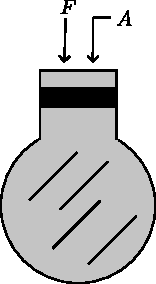
\includegraphics[scale=0.5]{te1.pdf}
  \caption{Presión}
  \label{te1}
\end{figure}

\begin{equation}
    p=\frac{F}{A}=\frac{N}{m^2}=Pa
\end{equation}

Si no hubiera gravedad, la presión siempre sería la misma, y a eso se le conoce como el \textbf{Principio de Pascal}

\begin{definition}[Principio de Pascal]
    La presión actuada a un fluido cerrado es transmitido intactamente a todos los puntos en el fluido y a las paredes del contenedor
\end{definition}


    %%%%%%%%%%%%%%%%%%%%%%%%%%%%%%%%%%%%%%%%%%%%%%%%%%%%%%%%%%%%%%%%%%%%%%%%%%%%%%%%%%%%%%%%%%%%%%%%%%%%%%%%%%%
    %%%%%%%%%%%%%%%%%%%%%%%%%%%%%%%%%%%%%%%%%%%%%%%%%%%%%%%%%%%%%%%%%%%%%%%%%%%%%%%%%%%%%%%%%%%%%%%%%%%%%%%%%%%
    \item Concepto de presión.
    
    \textit{sol. }
    Hay que tener claro que la presión es una medida escalar, y no tiene dirección, pero la fuerza lo tiene y estará perpendicularmente en el muro. Éste comportamiento puede expresarse matemáticamente como sigue:

\begin{equation}
    \lim_{x\to 0}\frac{\Delta F}{\Delta A}=P
\end{equation}
    %%%%%%%%%%%%%%%%%%%%%%%%%%%%%%%%%%%%%%%%%%%%%%%%%%%%%%%%%%%%%%%%%%%%%%%%%%%%%%%%%%%%%%%%%%%%%%%%%%%%%%%%%%%
    %%%%%%%%%%%%%%%%%%%%%%%%%%%%%%%%%%%%%%%%%%%%%%%%%%%%%%%%%%%%%%%%%%%%%%%%%%%%%%%%%%%%%%%%%%%%%%%%%%%%%%%%%%%
    \item Gato hidráulico. Principio de su operación y aplicaciones.
    
    \textit{sol. }
    
    Supongamos tener un contenedor con una forma característica como en la figura \ref{te2},
    
    \begin{figure}[h!]
  \centering
  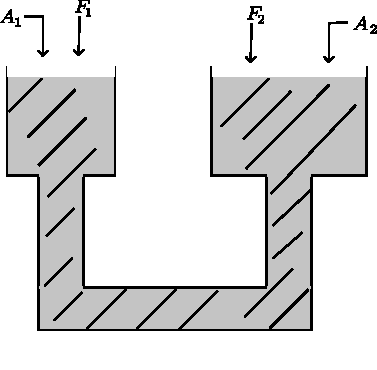
\includegraphics[scale=0.5]{te2.pdf}
  \caption{Gato Hidráulico}
  \label{te2}
\end{figure}

Por el principio de Pascal, la presión debe ser la misma, por lo que se puede plantear la siguiente relación:

\begin{equation*}
    \frac{F_1}{A_1}=\frac{F_2}{A_2}
\end{equation*}

    %%%%%%%%%%%%%%%%%%%%%%%%%%%%%%%%%%%%%%%%%%%%%%%%%%%%%%%%%%%%%%%%%%%%%%%%%%%%%%%%%%%%%%%%%%%%%%%%%%%%%%%%%%%
    %%%%%%%%%%%%%%%%%%%%%%%%%%%%%%%%%%%%%%%%%%%%%%%%%%%%%%%%%%%%%%%%%%%%%%%%%%%%%%%%%%%%%%%%%%%%%%%%%%%%%%%%%%%
    \item ¿Qué relación existe entre los trabajos de los extremos de gato hidráulico?
    
    \textit{sol. }
Si se aplica esa fuerza, entonces el fluido va a recorrer una distancia, que se le denotará $d_1$, entonces del otro lado también subirá una distancia $d_2$, esto implica que:

\begin{align*}
    &A_1d_1=A_2d_2\\
    &F_1d_1=F_2D_2
\end{align*}

Por ejemplo, se necesitaría el potencial de 100 metros para levantar un objeto del otro lado un sólo metro. 
%%%%%%%%%%%%%%%%%%%%%%%%%%%%%%%%%%%%%%%%%%%%%%%%%%%%%%%%%%%%%%%%%%%%%%%%%%%%%%%%%%%%%%%%%%%%%%%%%%%%%%%%%%
%%%%%%%%%%%%%%%%%%%%%%%%%%%%%%%%%%%%%%%%%%%%%%%%%%%%%%%%%%%%%%%%%%%%%%%%%%%%%%%%%%%%%%%%%%%%%%%%%%%%%%%%%%
    \item ¿Cómo tomar en cuenta la gravedad, y cómo se expresa, qué ecuación resulta?
    
    \textit{sol. }
La presciencia de alguna alteración a causa de la gravedad, es evidente cuando bajamos en el océano, la presión sube. Esto se puede demostrar con un diagrama como en la figura \ref{te3}:

    \begin{figure}[h!]
  \centering
  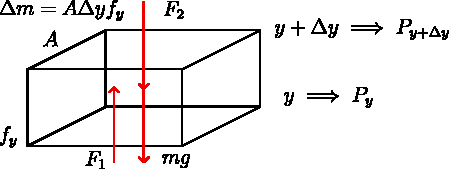
\includegraphics[scale=0.5]{te3.pdf}
  \caption{Fluido en equilibrio}
  \label{te3}
\end{figure}


    %%%%%%%%%%%%%%%%%%%%%%%%%%%%%%%%%%%%%%%%%%%%%%%%%%%%%%%%%%%%%%%%%%%%%%%%%%%%%%%%%%%%%%%%%%%%%%%%%%%%%%%%%%%
    %%%%%%%%%%%%%%%%%%%%%%%%%%%%%%%%%%%%%%%%%%%%%%%%%%%%%%%%%%%%%%%%%%%%%%%%%%%%%%%%%%%%%%%%%%%%%%%%%%%%%%%%%%%
    \item Las presiones verticales son perpendiculares a la superficie del elemento de fluido en equilibrio. Se usa para aplicar el balance de masa y ¿derivar qué?
    
    \textit{sol. }
    
    Del diagrama \ref{te3}, se puede plantear la siguiente ecuación igualada a cero, por estar en equilibrio:
    
    \begin{equation*}
        F_1-F_2-\Delta mg=0
    \end{equation*}
    
    Al mismo tiempo, se observa una relación:
\begin{align*}
&\stackbin[y]{}{PA}-\stackbin[y+\Delta y]{}{PA}-A\Delta y-\rho_yg=0\\
&\frac{P_{y+\Delta y}-P_y}{\Delta y}=-\rho_yg
\end{align*}

Si calculamos el límite

\begin{equation*}
    \lim_{\Delta y\to 0}\frac{P_{y+\Delta y}-P_y}{\Delta y}=-\rho_yg=\frac{dp}{dy}
\end{equation*}

Así se demuestra que cuando incrementamos el valor de $y$, la presión va a disminuir porque es un signo negativo. A esto se le conoce como \textbf{Presión Hidrostática }

    %%%%%%%%%%%%%%%%%%%%%%%%%%%%%%%%%%%%%%%%%%%%%%%%%%%%%%%%%%%%%%%%%%%%%%%%%%%%%%%%%%%%%%%%%%%%%%%%%%%%%%%%%%%
    %%%%%%%%%%%%%%%%%%%%%%%%%%%%%%%%%%%%%%%%%%%%%%%%%%%%%%%%%%%%%%%%%%%%%%%%%%%%%%%%%%%%%%%%%%%%%%%%%%%%%%%%%%%

    \item Diferencia entre gases y líquidos, aplicaciones de las propiedades de cada uno y cómo se explica. Describe el experimento, ¿qué concluyes?
    
    \textit{sol. }
    
    Los líquidos son incompresibles, eso significa que su densidad no varía a menos de inducirlo con presiones y fuerzas muy altas, por lo que podemos generalizar la ecuación como sigue.
    
    \begin{equation}
        -fg=\frac{dp}{dy}
    \end{equation}
    
    Pero los gases son comprensibles y por eso pueden variar la densidad.
    %%%%%%%%%%%%%%%%%%%%%%%%%%%%%%%%%%%%%%%%%%%%%%%%%%%%%%%%%%%%%%%%%%%%%%%%%%%%%%%%%%%%%%%%%%%%%%%%%%%%%%%%%%%
    %%%%%%%%%%%%%%%%%%%%%%%%%%%%%%%%%%%%%%%%%%%%%%%%%%%%%%%%%%%%%%%%%%%%%%%%%%%%%%%%%%%%%%%%%%%%%%%%%%%%%%%%%%%
    \item  Expresión matemática de la ley de Pascal, explicarla.
    
    \textit{sol. }
    
    Para demostrar la intuición de la presión en las latas, se procede a calcular el área con integrales siguiendo la lógica del diagrama \ref{te4}:
    
    \begin{figure}[h!]
      \centering
      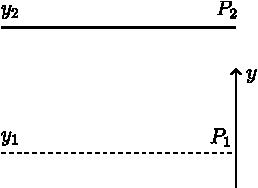
\includegraphics[scale=0.5]{te4.pdf}
      \caption{Ley de Pascal}
      \label{te4}
    \end{figure}

\begin{equation}
    \int^{P_2}_{P_1}dp=-\rho g\int^{y_2}_{y_1}dy
\end{equation}
    
    La cuestión es que $-\rho$ es una función de altitud en la atmósfera pero no con líquidos, por lo que se plantea como:
    
    \begin{equation*}
        P_2-P_1=-\rho g\left(y_2-y_1 \right)
    \end{equation*}
    
    Y acomodando los signos, obtenemos la \textbf{Ley de Pascal}:
    
    \begin{equation}
        P_1-P_2=\rho g\left(y_2-y_1 \right)
    \end{equation}
    %%%%%%%%%%%%%%%%%%%%%%%%%%%%%%%%%%%%%%%%%%%%%%%%%%%%%%%%%%%%%%%%%%%%%%%%%%%%%%%%%%%%%%%%%%%%%%%%%%%%%%%%%%%
    %%%%%%%%%%%%%%%%%%%%%%%%%%%%%%%%%%%%%%%%%%%%%%%%%%%%%%%%%%%%%%%%%%%%%%%%%%%%%%%%%%%%%%%%%%%%%%%%%%%%%%%%%%%

    \item  Consecuencias de la ley de Pascal...
    
    \textit{sol. }
    
        En la figura \ref{te5}, es un contenedor con un líquido que tiene una forma extraña, se llena hasta cierto punto y para medir la presión, se coloca un cilindro. Sin embargo la presión es distinta a lo largo y ancho del contenedor.
    
        \begin{figure}[h!]
      \centering
      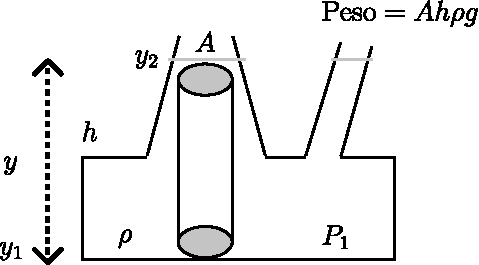
\includegraphics[scale=0.5]{te5.pdf}
      \caption{Vaso con dos salidas}
      \label{te5}
    \end{figure}
    
    %%%%%%%%%%%%%%%%%%%%%%%%%%%%%%%%%%%%%%%%%%%%%%%%%%%%%%%%%%%%%%%%%%%%%%%%%%%%%%%%%%%%%%%%%%%%%%%%%%%%%%%%%%%
    %%%%%%%%%%%%%%%%%%%%%%%%%%%%%%%%%%%%%%%%%%%%%%%%%%%%%%%%%%%%%%%%%%%%%%%%%%%%%%%%%%%%%%%%%%%%%%%%%%%%%%%%%%%

    \item  ¿Cómo describe la presión de la columna de aire y cómo se expresa?
    
    \textit{sol. }
    
    Si estamos a nivel del mar, y medimos la presión que hay en ese cilindro de $1cm^3$ de diámetro y con cientos de metros de distancia para alcanzar el límite, se observa que llegamos a:
    
    \begin{equation}
        1Kg/cm^2\approx 10^5Pa=1atm
    \end{equation}
    
    %%%%%%%%%%%%%%%%%%%%%%%%%%%%%%%%%%%%%%%%%%%%%%%%%%%%%%%%%%%%%%%%%%%%%%%%%%%%%%%%%%%%%%%%%%%%%%%%%%%%%%%%%%%
    %%%%%%%%%%%%%%%%%%%%%%%%%%%%%%%%%%%%%%%%%%%%%%%%%%%%%%%%%%%%%%%%%%%%%%%%%%%%%%%%%%%%%%%%%%%%%%%%%%%%%%%%%%%
    \item  Presión atmosférica, ¿es llamada presión?...
    
    \textit{sol. }
    
    \textbf{Presión Barométrica} gracias al barómetro, instrumento que mide las presión atmosférica
    
    %%%%%%%%%%%%%%%%%%%%%%%%%%%%%%%%%%%%%%%%%%%%%%%%%%%%%%%%%%%%%%%%%%%%%%%%%%%%%%%%%%%%%%%%%%%%%%%%%%%%%%%%%%%
    %%%%%%%%%%%%%%%%%%%%%%%%%%%%%%%%%%%%%%%%%%%%%%%%%%%%%%%%%%%%%%%%%%%%%%%%%%%%%%%%%%%%%%%%%%%%%%%%%%%%%%%%%%%
    \item  ¿Cómo se puede medir la presión atmosférica? si ``no la percibimos''
    
    \textit{sol. }
    
    Si se realiza un experimento que consiste en un vaso con un líquido e insertamos una manguera totalmente, y al descubrir un pedazo de ella, se revela que hay líquido en esa parte aún, pero esto es causa de la presión barométrica que la empuja hacia arriba siempre y cuando tapamos el orificio, pues de lo contrario bajará. 
    %%%%%%%%%%%%%%%%%%%%%%%%%%%%%%%%%%%%%%%%%%%%%%%%%%%%%%%%%%%%%%%%%%%%%%%%%%%%%%%%%%%%%%%%%%%%%%%%%%%%%%%%%%%
    %%%%%%%%%%%%%%%%%%%%%%%%%%%%%%%%%%%%%%%%%%%%%%%%%%%%%%%%%%%%%%%%%%%%%%%%%%%%%%%%%%%%%%%%%%%%%%%%%%%%%%%%%%%

    \item  ¿Qué derivación llevó a cabo para obtener la ecuación de la presión barométrica? Y ¿Cuál es la ecuación que obtuvo? ¿Quién lo hizo primero? el barómetro.
    
    \textit{sol. }
    
    Siguiendo el esquema \ref{te6}, se puede analizar la igualdad:
    
    \begin{equation*}
        P_1-P_2=\rho gh
    \end{equation*}
    
    \begin{figure}[h!]
      \centering
      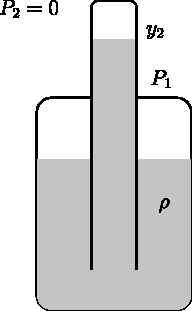
\includegraphics[scale=0.5]{te6.pdf}
      \caption{Barómetro}
      \label{te6}
    \end{figure}
    
    Pero realmente $P_2$ es cero, por lo que la presión Barométrica se expresa como:
    
    \begin{equation}
        P_1=\rho gh
    \end{equation}
    
    %%%%%%%%%%%%%%%%%%%%%%%%%%%%%%%%%%%%%%%%%%%%%%%%%%%%%%%%%%%%%%%%%%%%%%%%%%%%%%%%%%%%%%%%%%%%%%%%%%%%%%%%%%%
    %%%%%%%%%%%%%%%%%%%%%%%%%%%%%%%%%%%%%%%%%%%%%%%%%%%%%%%%%%%%%%%%%%%%%%%%%%%%%%%%%%%%%%%%%%%%%%%%%%%%%%%%%%%
    \item  ¿Cómo se describe la presión atmosférica?, con qué líquidos se pueden construir los barómetros.
    
    \textit{sol. }
    Torricelli descubrió que el mercurio tiene una densidad de $13.6\times 10^3Kg/cm^3$, la altura $h=0.76m$, reemplazando los datos, tenemos:
    
    \begin{equation*}
        P_1=\left( 13.6\times 10^3Kg/cm^3 \right)(0.76m)=1.03\times10^5Pa
    \end{equation*}
    
    Un resultado muy aproximado al que se tomó en cuenta de $1Kg/cm^2$. 
    
    
    %%%%%%%%%%%%%%%%%%%%%%%%%%%%%%%%%%%%%%%%%%%%%%%%%%%%%%%%%%%%%%%%%%%%%%%%%%%%%%%%%%%%%%%%%%%%%%%%%%%%%%%%%%%
    %%%%%%%%%%%%%%%%%%%%%%%%%%%%%%%%%%%%%%%%%%%%%%%%%%%%%%%%%%%%%%%%%%%%%%%%%%%%%%%%%%%%%%%%%%%%%%%%%%%%%%%%%%%
    \item  ¿10 m de columna de agua es equivalente a qué?
    
    \textit{sol. }
    
    A un barómetro de agua para medir una atmósfera. Sin embargo a esto se le llama \textbf{Presión Hidrostática}.
    
    
    %%%%%%%%%%%%%%%%%%%%%%%%%%%%%%%%%%%%%%%%%%%%%%%%%%%%%%%%%%%%%%%%%%%%%%%%%%%%%%%%%%%%%%%%%%%%%%%%%%%%%%%%%%%
    %%%%%%%%%%%%%%%%%%%%%%%%%%%%%%%%%%%%%%%%%%%%%%%%%%%%%%%%%%%%%%%%%%%%%%%%%%%%%%%%%%%%%%%%%%%%%%%%%%%%%%%%%%%
    \item  ¿Cómo se calcula presión hidrostática en el agua y cómo cambia con la profundidad?
    
    \textit{sol. }
    
Partiendo de que en todos los puntos sobre el fluido se encuentran en equilibrio, la presión hidrostática es directamente proporcional a la densidad del líquido, a la profundidad y a la gravedad.
    %%%%%%%%%%%%%%%%%%%%%%%%%%%%%%%%%%%%%%%%%%%%%%%%%%%%%%%%%%%%%%%%%%%%%%%%%%%%%%%%%%%%%%%%%%%%%%%%%%%%%%%%%%%
    %%%%%%%%%%%%%%%%%%%%%%%%%%%%%%%%%%%%%%%%%%%%%%%%%%%%%%%%%%%%%%%%%%%%%%%%%%%%%%%%%%%%%%%%%%%%%%%%%%%%%%%%%%%
    \item  ¿A cuántos metros de profundidad en el agua, se tiene una presión igual a la que produce la atmósfera en la superficie de la tierra? ¿Qué espesor, aproximado, tiene la atmósfera?
    
    \textit{sol. }
        
    Si se bajan 100 metros de profundidad en el océano, entonces la presión hidrostática se incrementa por diez atmósferas, osea que por cada diez metros de profundidad, es equivalente a una atmósfera. 
    
    %%%%%%%%%%%%%%%%%%%%%%%%%%%%%%%%%%%%%%%%%%%%%%%%%%%%%%%%%%%%%%%%%%%%%%%%%%%%%%%%%%%%%%%%%%%%%%%%%%%%%%%%%%%
    %%%%%%%%%%%%%%%%%%%%%%%%%%%%%%%%%%%%%%%%%%%%%%%%%%%%%%%%%%%%%%%%%%%%%%%%%%%%%%%%%%%%%%%%%%%%%%%%%%%%%%%%%%%
    \item  ¿Qué aplicación tiene el conocimiento de la presión para la construcción y operación de los submarinos?
    
    \textit{sol. }
    
    El primer submarino tenía la capacidad de bajar cinco metros de profundidad en el agua, esto implica que carga una presión de media atmósfera; sin embargo, como ellos bajaban una presión de una atmósfera, era posible soportar la fuerza perpendicular que se somete.
    
    %%%%%%%%%%%%%%%%%%%%%%%%%%%%%%%%%%%%%%%%%%%%%%%%%%%%%%%%%%%%%%%%%%%%%%%%%%%%%%%%%%%%%%%%%%%%%%%%%%%%%%%%%%%
    %%%%%%%%%%%%%%%%%%%%%%%%%%%%%%%%%%%%%%%%%%%%%%%%%%%%%%%%%%%%%%%%%%%%%%%%%%%%%%%%%%%%%%%%%%%%%%%%%%%%%%%%%%%

    \item  ¿Qué aplicación para el buceo? Explíquelo. Snorkel (¿qué pasa?), ¿qué tan profundo lo puedes hacer?
    
    \textit{sol. }
    
    
    Suponiendo que bajamos tan solo 10 metros de la superficie, no podríamos respirar en el tubo, pues éste sería además de largo, se cuenta con una presión de dos atmósfera, pero en la superficie hay una atmósfera, por lo que se necesita mucha fuerza para poder respirar.
    
    %%%%%%%%%%%%%%%%%%%%%%%%%%%%%%%%%%%%%%%%%%%%%%%%%%%%%%%%%%%%%%%%%%%%%%%%%%%%%%%%%%%%%%%%%%%%%%%%%%%%%%%%%%%
    %%%%%%%%%%%%%%%%%%%%%%%%%%%%%%%%%%%%%%%%%%%%%%%%%%%%%%%%%%%%%%%%%%%%%%%%%%%%%%%%%%%%%%%%%%%%%%%%%%%%%%%%%%%
    \item  ¿Qué presión debe hacerse con los pulmones para contrarrestar la presión atmosférica?
    
    \textit{sol. }
    Se necesitaría una atmósfera más, porque en la superficie hay dos y en la parte inferior sólo una, pero se necesitaría un tanque de oxígeno a presión.
    %%%%%%%%%%%%%%%%%%%%%%%%%%%%%%%%%%%%%%%%%%%%%%%%%%%%%%%%%%%%%%%%%%%%%%%%%%%%%%%%%%%%%%%%%%%%%%%%%%%%%%%%%%%
    %%%%%%%%%%%%%%%%%%%%%%%%%%%%%%%%%%%%%%%%%%%%%%%%%%%%%%%%%%%%%%%%%%%%%%%%%%%%%%%%%%%%%%%%%%%%%%%%%%%%%%%%%%%
    \item  ¿Qué es un manómetro? y ¿Qué mide, cómo se deriva la ecuación para cuantificar la presión?
    
    \textit{sol. }
    
    Un manómetro es un instrumento para medir la presión de fluidos contenidos en recipientes cerrados, como en la figura \ref{te7}.
    
    
    \begin{figure}[h!]
      \centering
      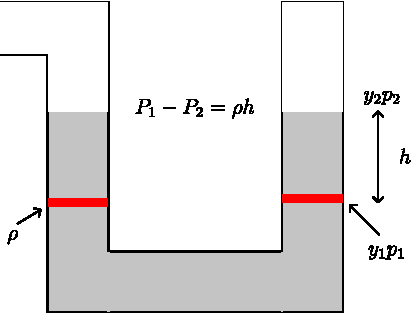
\includegraphics[scale=0.5]{te7.pdf}
      \caption{Manómetro}
      \label{te7}
    \end{figure}
    
    Como $P_2$ en éste caso vale una atmósfera, entonces podemos finalizar la formula:
    \begin{equation}
        P_1=1atm+\rho hg
    \end{equation}
\end{enumerate}

Podemos enumerar algunas ideas principales:

\begin{enumerate}
    \item La propiedad fundamental que caracteriza a los fluidos (líquidos y gases) es que carecen de rigidez y en consecuencia se deforman fácilmente. Por este motivo un fluido no tiene forma y diferentes porciones del mismo se pueden acomodar dentro del recipiente que lo contiene. En esto
difieren de los sólidos, que en virtud de su rigidez tienen una forma definida, que sólo varía si se aplican fuerzas de considerable intensidad.
\item EL principio de Pascal puede enunciarse como`` la presión ejercida sobre un fluido incompresible y en equilibrio dentro de un recipiente de paredes indeformables se transmite con igual intensidad en todas las direcciones y en todos los puntos del fluido.''
\item La presión atmosférica es la fuerza por unidad de superficie que ejerce el aire que forma la atmósfera sobre la superficie terrestre.
\item La presión hidrostática es la parte de la presión debida al peso de un fluido en reposo. En un fluido en reposo la única presión existente es la presión hidrostática, en un fluido en movimiento puede aparecer una presión hidrodinámica adicional relacionada con la velocidad del fluido. 
\end{enumerate}













